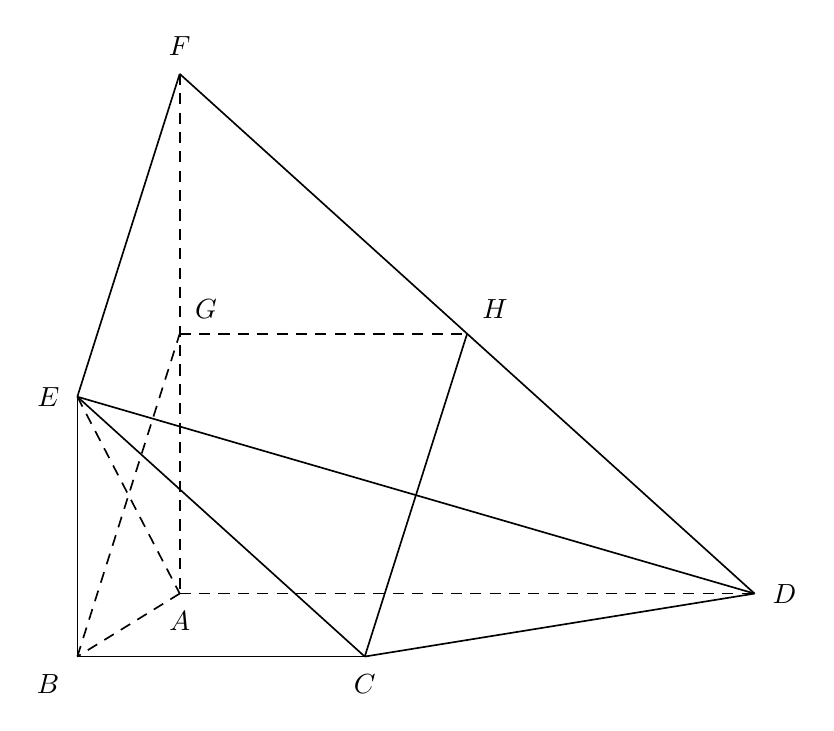
\begin{tikzpicture}[x=1cm,y=1cm,font=\normalsize,
  edge/.style={draw=black,solid,line width=.6pt},
  hid/.style={draw=black,dashed,line width=.6pt,dash pattern=on 4pt off 3pt},
  lbl/.style={font=\normalsize,inner sep=1.5pt}]
% Vertices of the two right-trapezoid solid (schematic projection).
\coordinate (F) at (1.3000000000,8.4000000000);
\coordinate (E) at (0.0000000000,4.3000000000);
\coordinate (B) at (0,1.0);
\coordinate (A) at (1.3,1.8);
\coordinate (C) at (3.6500000000,1.0000000000);
\coordinate (D) at (8.6,1.8);
% Midpoints G on FA and H on FD (exact by construction below).
\coordinate (G) at (1.3000000000,5.1000000000);
\coordinate (H) at (4.9500000000,5.1000000000);
% Visible edges.
\draw[edge] (F)--(E);
\draw[edge] (F)--(H);
\draw[edge] (H)--(D);
\draw[edge] (E)--(B);
\draw[edge] (E)--(C);
\draw[edge] (E)--(D);
\draw[edge] (B)--(C);
\draw[edge] (C)--(D);
\draw[edge] (H)--(C);
% Hidden edges.
\draw[hid] (F)--(A);
\draw[hid] (E)--(A);
\draw[hid] (A)--(B);
\draw[hid] (A)--(D);
\draw[hid] (B)--(G);
\draw[hid] (G)--(H);
% Labels placed clear of all strokes.
\node[above=3pt] at (F) {$F$};
\node[left=3pt] at (E) {$E$};
\node[below left=3pt] at (B) {$B$};
\node[below=3pt] at (A) {$A$};
\node[below=3pt] at (C) {$C$};
\node[right=3pt] at (D) {$D$};
\node[above right=2pt] at (G) {$G$};
\node[above right=2pt] at (H) {$H$};
\end{tikzpicture}
